\subsection{Drivers' Responses to These Patterns}
Investigating driver responses, we find no correlation between daily work hours and concurrent average PM2.5 levels
% \mick{removed fig}.
(\autoref{fig:work-hours-vs-aqi-per-rider}).
This lack of temporal adjustment aligns with qualitative findings where drivers perceive pollution exposure as an unavoidable occupational hazard, often prioritizing immediate income over avoiding polluted times or areas if it means lost earnings, echoing sentiments like pollution being ``everywhere anyway'' (BKK-1) or avoiding smoggy areas meaning driving an ``empty car out'' (BKK-5).
This resignation, where enduring poor air is ``simply something they have to be able to live with'' (BKK-4),
mirrors observations in gig work research regarding the normalization of health risks under precarious conditions.
However, despite not altering schedules, spatial analysis
\mick{removed fig}
%(\autoref{fig:location-bin-hour})
reveals drivers spend the majority of their time in subdistricts with lower PM2.5 levels (below 100 $\mu g / m^3$).
% This suggests a potential spatial adaptation: while not reducing work hours due to pollution, drivers appear to select service locations favoring relatively lower exposure,
% \joe{i dont think you can say this. does qualitative findings show this?}
% possibly because location choices can be adjusted with less direct income penalty than restricting work hours.

To investigate the drivers' response to PM 2.5 level, we create
\mick{removed fig}
% \autoref{fig:daily-work-hour-per-driver}
\joe{really weird way to say this... change to something like "Fig. N Shows..."}comparing drivers' working time throughout the period of the study.
Despite the air pollution exposure to these drivers in \autoref{fig:daily-pollution-per-driver} shows patterns with clear peaks during certain time periods,
\todo{The drivers' working time in
\mick{removed fig}
% \autoref{fig:daily-work-hour-per-driver}
does not present any pattern.}
To look further into daily routine of each participant,
we visualize scatter plots showing relationships between each driver's work hours in each day and the average PM2.5 measured on that day.
Unfortunately \joe{also weird. state results as facts not as sentiment... no "unfortunately"}\kurtis{concur}, we do not find correlation between these two variables for any of the participants.

As expected from previous research, our participants expressed similar perceptions regarding air pollution. Many drivers viewed exposure to hazardous air as an unavoidable aspect of their profession rather than a modifiable risk \cite{tieanklin2024rideshare}. 
As most of our participants reflected,

\begin{quoteb}
    ``I just go where the application tells me to go,...,the (air) pollution is everywhere anyway '' (BKK-1)
\end{quoteb}

Oftentimes they are restricted by the income that they would make that day as BKK-5 iterated his thought process in avoiding highly polluted areas,

\begin{quoteb}
    ``When I see that the area gets smoggier, I often have thoughts about driving out to the suburban area. But that means I'll have to drive an empty car out'' (BKK-5)
\end{quoteb}


This emphasizes that enduring poor air quality was simply part of the job. BKK-4 driver echoed this sentiment by summarizing how drivers would feel about prioritizing their health stating, 

\begin{quoteb}
    ``People who choose to become (motorcycle taxi) drivers, they know what they get themselves into. Pushing through rains or pollution is simply just something they have to be able to live with.'' (BKK-4)
\end{quoteb}

This simply suggests a sense of resignation rather than an expectation of change. 
This aligns with broader findings in gig work research, where workers in precarious conditions often normalize health risks as an occupational necessity.

On the other hand, location may not necessarily affect the drivers' income directly, so adjusting the location of their driving service can be done more easily than restricting their work hours, given their income restriction.
As shown in, 
\mick{remove fig}
% \autoref{fig:location-bin-hour},
driver spent their majority of their time in the subdistricts where the PM 2.5 levels are below 50 $\mu g / m^3$.
This results indicate that drivers choose their service location in a way that avoid locations with high PM 2.5 levels.

% \begin{figure*}
%     \centering
%     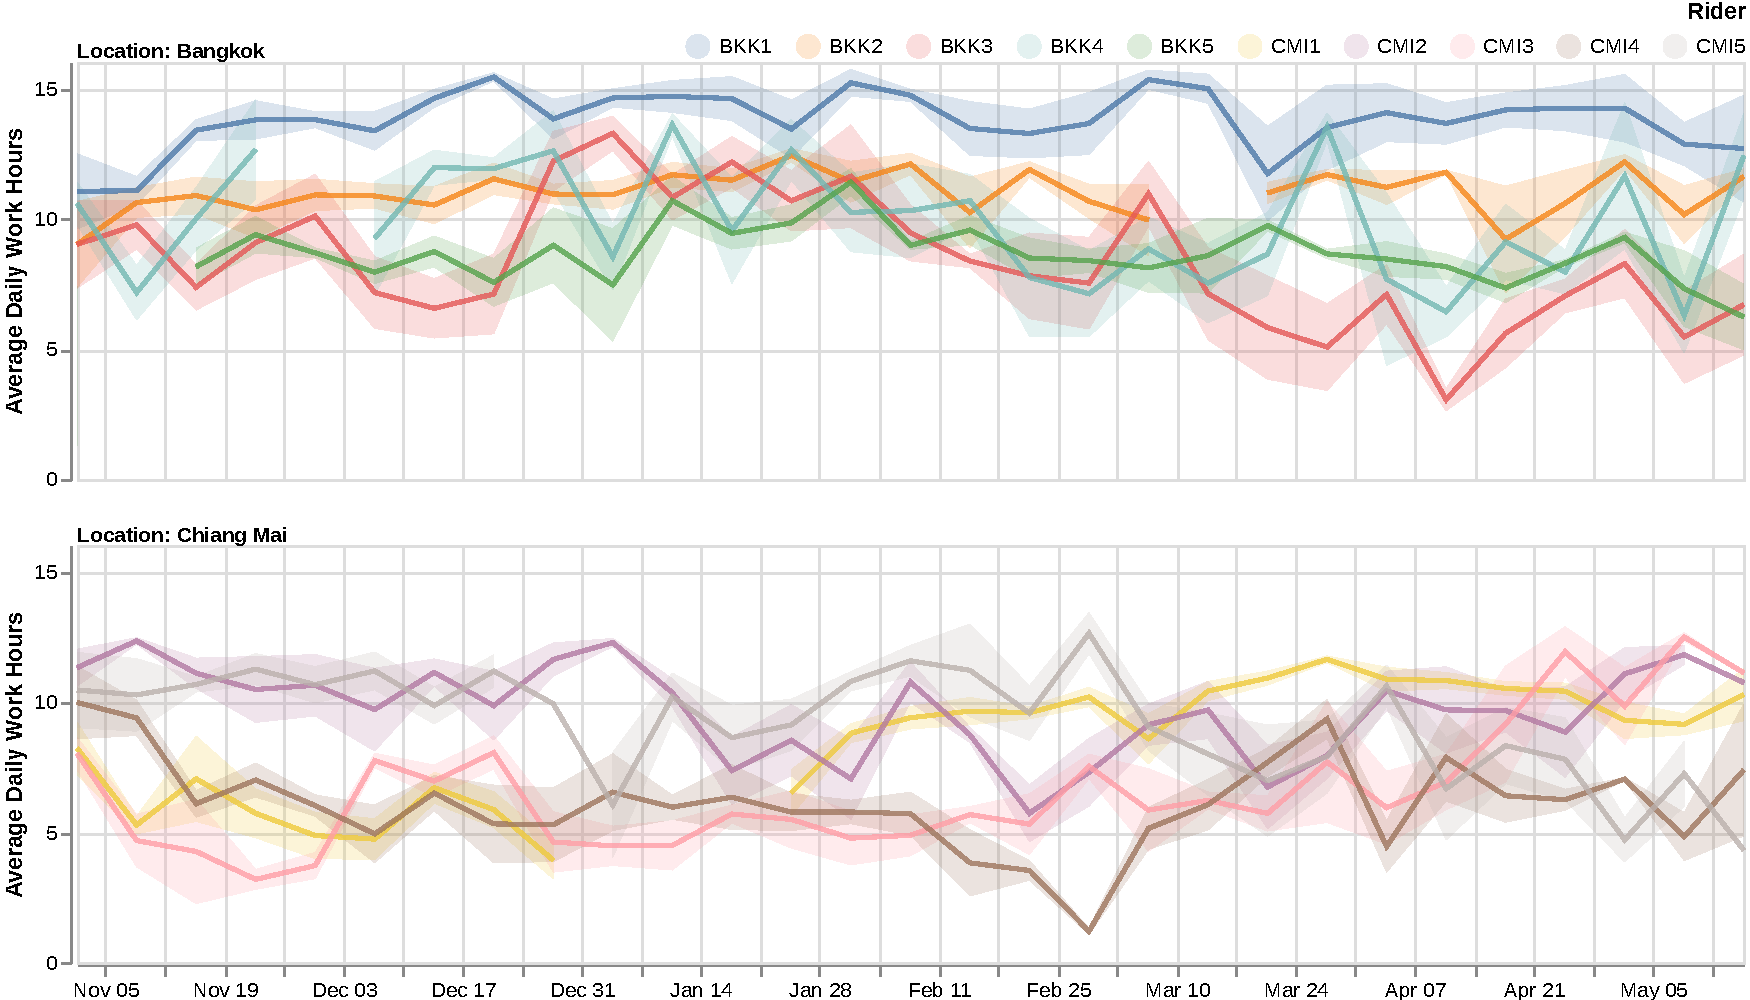
\includegraphics[width=\textwidth]{figures/weekly-work-hours-per-rider.pdf}
%     \caption{
%     Average daily working hours throughout each week collected from the helmet-mounted sensors for each driver from Bangkok and Chiang Mai.
%     The bands denote $\pm 1$ standard deviation from the average daily working hours throughout each week.\joe{why does this plot matter?}
%     % \kurtis{not understanding why these are a range}
%     % \joe{weekly working hours are only 10 hours per week? seems counter-intuitive to claims made previously that driver work long hours.}
%     }
%     \Description{}
%     \label{fig:daily-work-hour-per-driver}
% \end{figure*}%

% \begin{figure*}
%     \centering
%     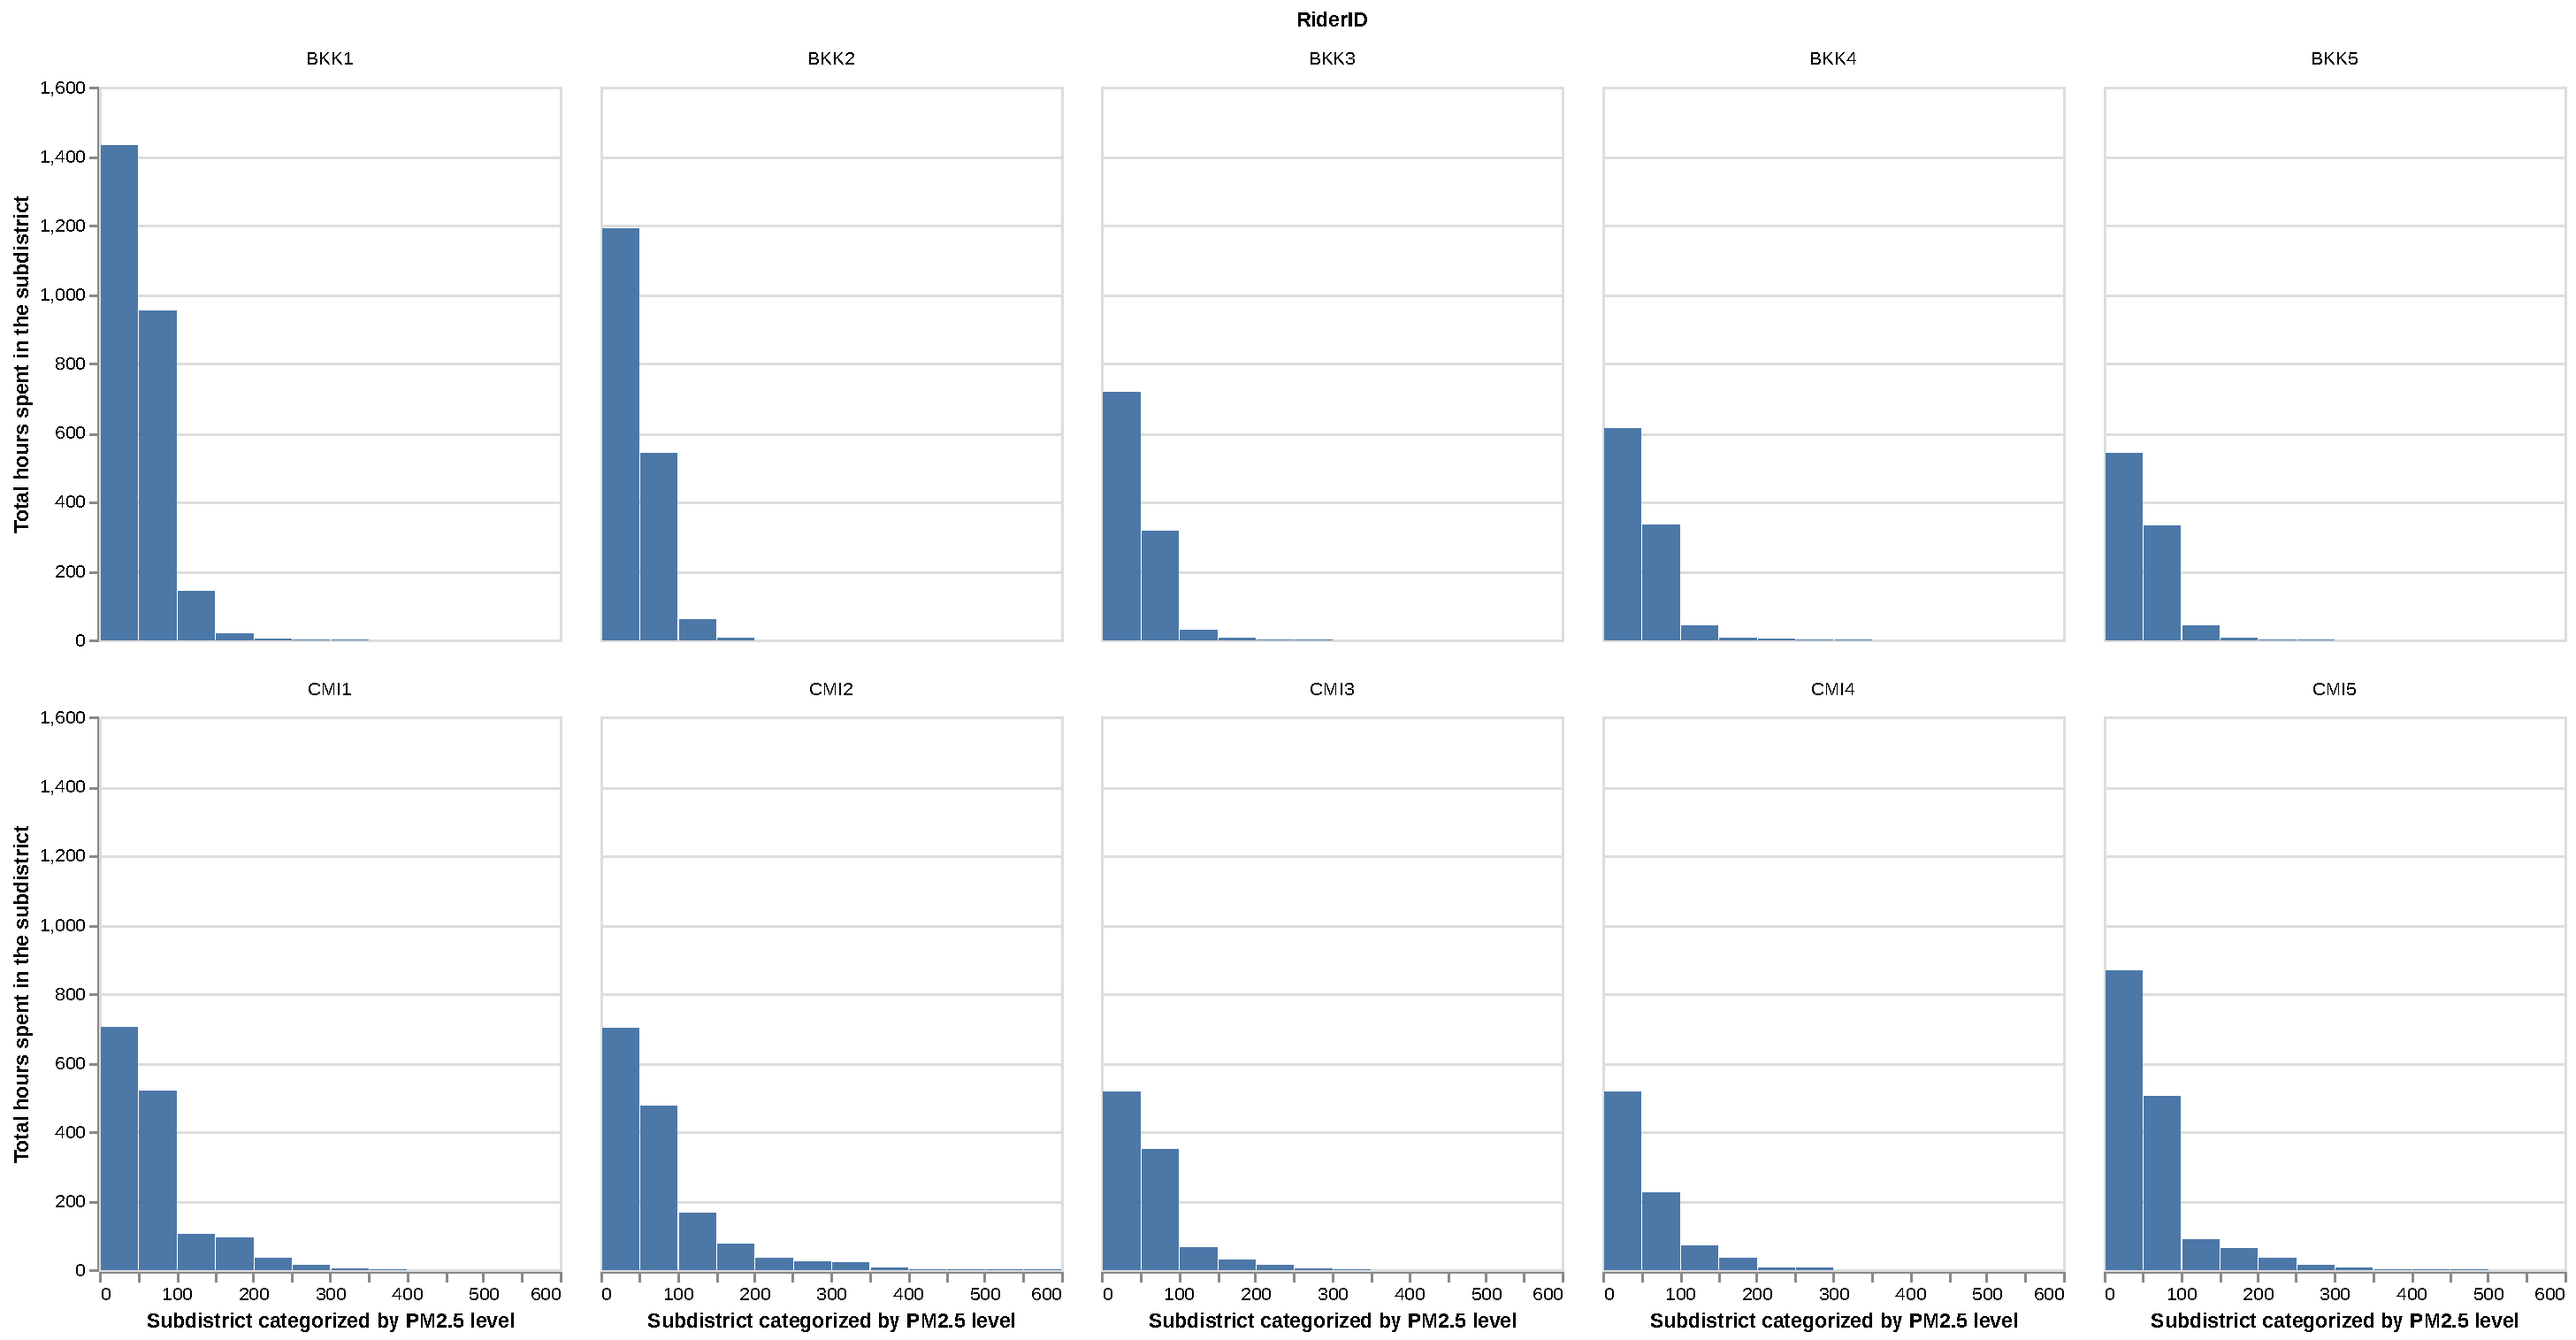
\includegraphics[width=\textwidth]{figures/location-bar-hour-work.pdf}
%     \caption{Bar charts showing total hours a driver spent throughout the study in subdistricts categorized by their measured PM 2.5 levels. \joe{why does this plot matter? Seems like it can be entirely omitted.}}
%     \Description{}
%     \label{fig:location-bin-hour}
% \end{figure*}

\paragraph{Answer to QS3}
While the drivers do not adjust their working schedule based on their observed air pollution, they are able to make inform decision to locations with high PM 2.5 levels and operate their services in the ares with relatively lower air pollution.

\begin{figure*}
    \centering
    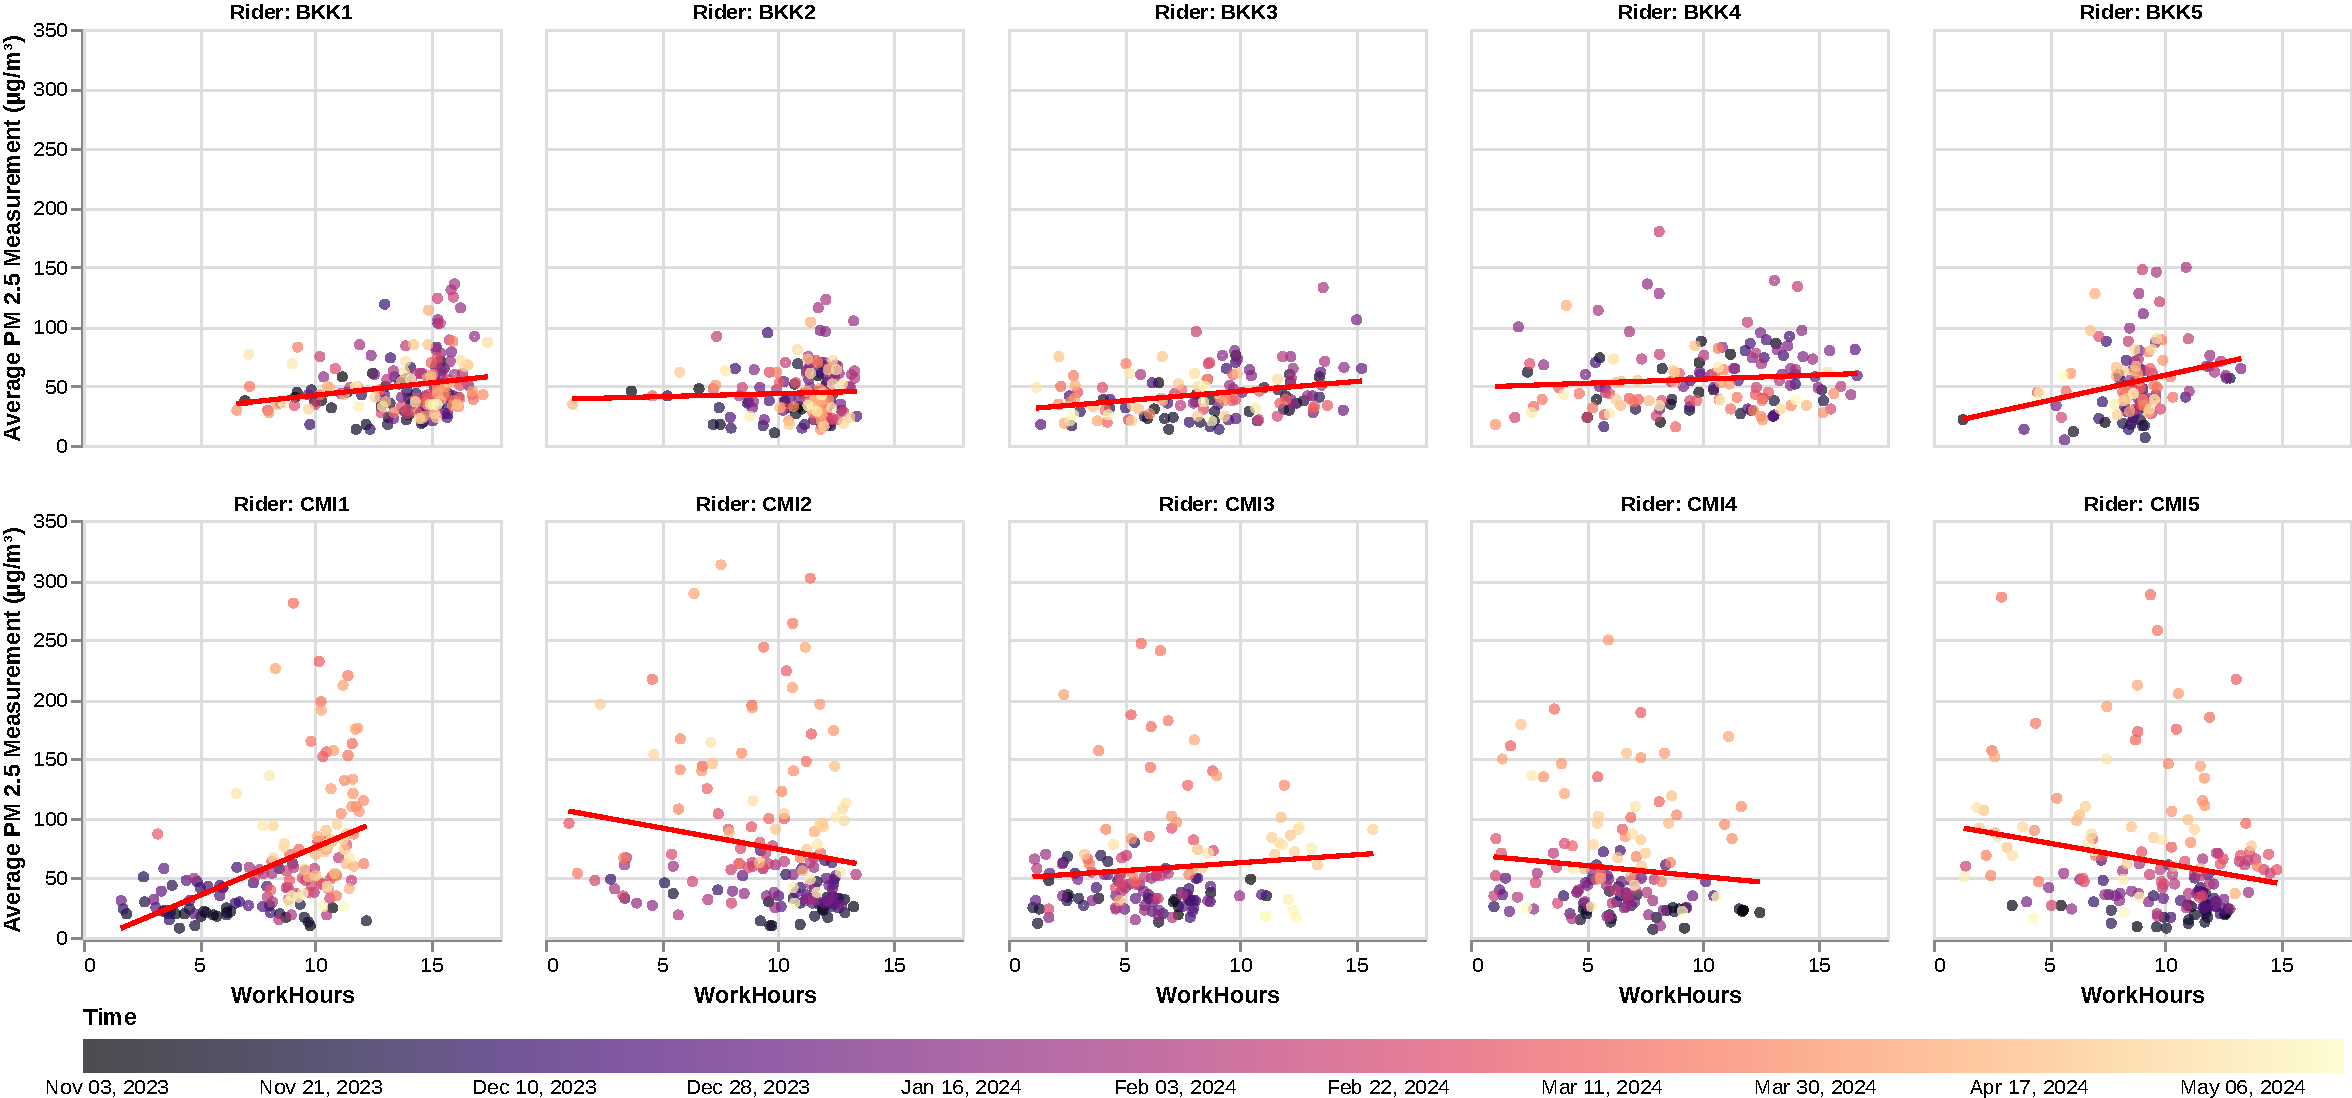
\includegraphics[width=\textwidth]{figures/work-hours-vs-aqi-per-rider-regression.pdf}
    \caption{Correlation of daily work hours and air pollution measurement for each driver, averaged through each week, with regression lines.
    % \joe{why are we aggregating to a weekly scale if we have daily data? A scatterplot is literally the perfect opportunity to represent disaggregated data and based on the fact that so many plots in this paper are per-participant, it seems like you wnat to show as fine grained data as possible?}
    }
    \Description{}
    \label{fig:work-hours-vs-aqi-per-rider}
\end{figure*}

% This section shows our results from analyzing data records collected from the helmet-mounted sensor.
% Our analytics are motivated by the following questions.
% \mick{relationships -- (aqi, time), (aqi, location), (aqi, time, location), time -> day of the year / day of the month, day of the week, hour of the day}
% \kurtis{aren't the rq in the intro?}
% \kurtis{i personally like phrasing things in terms of the driver's experiences; though the hour is late on big rewrites}
% \begin{enumerate}
%     \item[Q1] {\em Pollution Exposure Patterns}: How are the pollution exposure patterns for riders in general based on different time frames and locations \joe{too general. this is two questions: 1) does pollution exposure correlate spatially across different locations (importantly do different drivers see the same relative change in pollution exposure at the same locations?) 2) does pollution exposure correlate temporally across different times of the day or seasons? (i.e., worse during peak traffic hours? worse during certain seasons?) There is maybe a 3rd question of whether there are temporal patterns at specific locations and not at others. For instance, does PM2.5 in central neighborhoods fluccuate with traffic (time of day) but remains constant in residential neighborhoods?}?
%     \item[Q2] {\em Overall Driving Patterns}: What are riders' driving patterns based on air pollution and locations \joe{again, driver patterns vs location is one questions, driver patterns vs pollution is another question}?
%     % \item[Q3] {\em Comparison of Individual Driving Patterns}: When looking at each rider individually, how do they compare with each other? \firn{to remove - this will be answered in section mixed}
% \end{enumerate}